\documentclass[aspectratio=169]{beamer}
\usetheme{metropolis}

\usepackage{roboto}
\usepackage{mathtools}
\usepackage{fixmath}
\usepackage{graphicx}
\usepackage{tikz}
\usepackage{stmaryrd}

\graphicspath{ {./images/} }
\setbeamertemplate{navigation symbols}{}

\newcommand{\cntxt}{\ \mathrm{context}}
\newcommand{\typ}{\ \mathrm{type}}
\newcommand{\N}{\mathbb{N}}
\newcommand{\app}[2]{App_{[x:\sigma]\tau}(#1, #2)}
\newcommand{\pair}[2]{Pair_{[x:\sigma]\tau}(#1, #2)}
\newcommand{\R}[2]{\mathbold{R}_{[z:\Sigma x:\sigma.\tau]\rho}^{\Sigma}(#1, #2)}
\newcommand{\RN}[3]{\mathbold{R}_{[n: \N]\sigma}^{\N}(#1, #2, #3)}
\newcommand{\C}{Comp}
\newcommand{\Intro}{Intro}
\newcommand{\F}{Form}
\newcommand{\E}{Elim}
\newcommand\defeq{\stackrel{\mathclap{\normalfont\mbox{def}}}{\ =\ }}
\newcommand{\soundness}{\stackrel{\mathclap{\normalfont\mbox{$s$}}}{\ \implies\ }}
\newcommand{\Id}[2]{Id_\sigma(#1,#2)}
\newcommand{\Refl}[1]{Refl_\sigma(#1)}
\newcommand{\RID}[4]{\mathbold{R}_{[x:\sigma,y:\sigma,p:Id_\sigma(x,y)]\tau}^{Id}(#1, #2, #3, #4)}
\newcommand{\bn}{[n:\N,x:\sigma]}
\newcommand{\bi}{[z:\sigma]}
\newcommand{\Pich}{\hat{\Pi}}
\newcommand{\Appch}[2]{\hat{App}_{[x:\sigma]El(T)}(#1,#2)}
\newcommand{\lambdach}{\hat{\lambda} x:\sigma.M^{El(T)}}
\newcommand{\Gamdash}{\Gamma\vdash}
\newcommand{\Fami}{\mathcal{F}am}
\newcommand{\cate}{\mathcal{C}}
\newcommand{\types}{Ty_{\cate}}
\newcommand{\terms}{Tm_{\cate}}
\newcommand{\defin}[1]{\emph{\underline{#1}}}
\newcommand{\xsigmas}{x_1:\sigma_1, ..., x_n:\sigma_n}
\newcommand{\zthetas}{z_1:\theta_1, ..., z_n:\theta_n}
\newcommand{\pp}{\texttt{p}}
\newcommand{\qq}{\texttt{q}}
\newcommand{\vv}{\texttt{v}}
\newcommand{\extension}{\Gamma.\sigma}
\newcommand{\textension}{\langle f,M\rangle_\sigma}
\newcommand{\Mbar}{\overline{M}}

\DeclarePairedDelimiter\Brackets{\llbracket}{\rrbracket}

\title{Syntax and Semantics of Dependant Types}
\subtitle{by Martin Hofmann}
\author{Louis Milhaud}
\institute{Université Paris Saclay}
\date{\today}

\begin{document}

    \AtBeginSection[]{
    \begin{frame}
    \vfill
    \centering
    \begin{beamercolorbox}[sep=8pt,center,shadow=true,rounded=true]{title}
        \usebeamerfont{title}\insertsectionhead\par%
    \end{beamercolorbox}
    \vfill
    \end{frame}
    }
    % frame 1
    \begin{frame}
        \titlepage
    \end{frame}

    % frame 2
    \begin{frame}
        \frametitle{Outline}
        \tableofcontents
    \end{frame}

    % frame 3
    \section{Introduction}
    % frame 4
    \begin{frame}
        \frametitle{Definition}
        A dependant type is a family of types varying on the elements of another type.\\
        \vspace{20pt}
        \underline{Exemple:}\\
        $$Vec_\sigma(M),\quad M:\N $$
        Built on:
        \begin{itemize}
            \item $nil_\sigma : Vec_\sigma(0)$
            \item $Cons_\sigma(U, V) : Vec_\sigma(Succ(M))$ 
        \end{itemize}
        with $ U : \sigma\ \text{ and } V : Vec_\sigma(M)$
    \end{frame}

    \subsection{Syntax}
    % frame 5
    \begin{frame}
        \frametitle{Syntax}
        \begin{align*}
            \Gamma ::=\ &\diamond\\
                &|\ \Gamma,x:\sigma \qquad\text{provided $x$ is not declared in $\Gamma$}\\
                &\text{}\\
            \sigma,\tau ::=\ &\Pi x:\sigma.\tau\ |\ \Sigma x:\sigma.\tau\ |\ \Id{M}{N}\ |\ \N\\
            &\text{}\\
            M,N,H,P ::=\ &x\ |\ \lambda x:\sigma.M^\tau\ |\ \app{M}{N}\ |\ \pair{M}{N}\\
                &|\ \R{[x:\sigma,y:\tau]H}{M}\ |\ \Refl{M}\\
                &|\ \RID{[z:\sigma]H}{M}{N}{P}\ |\ 0\ |\ Suc(M)\ |\\
                &\RN{H_z}{[n:\N,x:\sigma]H_s}{M}
        \end{align*}
    \end{frame}

    \subsection{Term model}
    % frame 6
    \begin{frame}
        \frametitle{Context morphisms}
        Let $\Gamma$ and $\Delta \defeq x_1:\sigma_1,...,x_n:\sigma_n$ be valid contexts.\\
        $f \defeq (M_1,...,M_n)$ is a context morphism (we write $\Gamdash f \implies \Delta$)\\
        when the following $n$ judgements hold:
        \begin{align*}
            &\Gamdash M_1:\sigma_1\\
            &\Gamdash M_2:\sigma_2[M_1/x_1]\\
            &\dots\\
            &\Gamdash M_n:\sigma_n[M_1/x_1][M_2/x_2]\dots[M_{n-1}/x_{n-1}]
        \end{align*}
    \end{frame}

    % frame 7
    \begin{frame}
        \frametitle{Generalized substitution \& Composition}
        If we have:
        \begin{align*}
            \vdash \Gamma,\,\Delta\ &\cntxt\quad\Gamdash \tau \typ\\
            &\Gamdash f \implies \Delta\\
            &f \equiv (M_1, ..., M_n)\\
            &\Delta \equiv \xsigmas
        \end{align*}
        Then:
        $$\tau[f\slash\Delta]\equiv\tau[M_1\slash x_1][M_2\slash x_2]...[M_n\slash x_n]$$
        \vspace{8pt}\\
        Thanks to \textbf{substitution} we can now define context morphism \textbf{composition}:
        $$\text{Let }\Delta\vdash g\implies\Theta\text{ a context morphism, with }g\equiv(N_1,...,N_k)$$
        $$f \circ g\equiv(N_1[f\slash\Delta],...,N_k[f\slash\Delta])$$
    \end{frame}

    % frame 8
    \section{Semantic frameworks}
    \subsection{Categories with Famillies (CwF)}

    % frame 9
    \begin{frame}
        \frametitle{Objects}
        Let's first define some data structures in our \textbf{semantic model}:
        \vspace{8pt}
        \begin{itemize}
            \item $\cate$ category of contexts and context morphisms
            \vspace{8pt}
            \item for $\Gamma\in\cate$ a collection $\types(\Gamma)$ of semantic types
            \vspace{8pt}
            \item for $\Gamma\in\cate$ and $\sigma\in\types$ a collection $\terms(\Gamma,\sigma)$ of semantic terms
        \end{itemize}
    \end{frame}
    
    % frame 10
    \begin{frame}
        \frametitle{Context formation \& type extension}
        \emph{Formation:}
        \begin{itemize}
            \item $\top$ a \textbf{terminal} object in $\cate$
            \item $\forall \Gamma \in \cate,\ \langle\rangle_\Gamma$ denotes the unique morphism from $\Gamma$ to $\top$ 
        \end{itemize}
        \vspace{15pt}
        \emph{Type Extension:}
        \begin{itemize}
            \item $\forall (\Gamma,\sigma) \in \cate \times \types(\Gamma),\ \extension\in\cate$ is the \textbf{comprehension} of $\sigma$
            \item in the term model:
            $$\frac{\vdash\Gamma \cntxt\quad\Gamdash\sigma\typ}{\Gamma,x:\sigma\cntxt}$$
        \end{itemize}
    \end{frame}

     % frame 11
     \begin{frame}
        \frametitle{Substitution}
        \vspace{10pt}
        Semantic substitution is described by one operation for types and one for terms.\\
        \vspace{8pt}
        Let $f: \Gamma\to\Delta$, $g: \Delta\to\Theta$, $\sigma\in Ty(\Theta)$ and $M\in Tm(\Theta,\sigma)$
        \begin{itemize}
            \item $-\{g\}: Ty(\Theta)\to Ty(\Delta)$
            \item $-\{g\}:Tm(\Theta,\sigma)\to Tm(\Delta,\sigma\{g\})$
            \item compatible with composition and identities:
        \end{itemize}
        \begin{alignat*}{2}
            \sigma\{id_\Theta\} &= \sigma &&\in Ty(\Theta)\\
            \sigma\{g\circ f\} &= \sigma\{g\}\{f\} &&\in Ty(\Gamma)\\
            M\{id_\Theta\} &= M &&\in Tm(\Theta,\sigma)\\
            M\{g\circ f\} &= M\{g\}\{f\} &&\in Tm(\Gamma,\sigma\{g\circ f\})
        \end{alignat*}
    \end{frame}

    % frame 12
    \begin{frame}
        \frametitle{$\pp$ \& $\vv$ Morphisms}
        $\pp$ \emph{morphism:}
        \begin{itemize}
            \item $\pp(\sigma):\extension\to\Gamma$ is the projection associated to $\sigma$
            \item in the term model:
            $$\Gamma,x:\sigma\vdash\pp\implies\Gamma$$
        \end{itemize}
        \vspace{8pt}
        $\vv$ \emph{morphism:}
        \begin{itemize}
            \item $\vv_\sigma \in \terms(\extension,\sigma\{\pp(\sigma)\})$ is the second projection
            \item in the term model:
            $$\Gamma,x:\sigma\vdash x:\sigma$$
        \end{itemize}
    \end{frame}

    % frame 13
    \begin{frame}
        \frametitle{Term Extension}
        \vspace{15pt}
        Let $f:\Gamma\to\Delta,\ \sigma\in Ty(\Delta)$ and $M\in Tm(\Gamma,\sigma\{f\})$.
        \begin{itemize} 
            \item $\textension:\Gamma\to\Delta.\sigma$ is the extension of $f$ by $M$
            \item if $g:\Theta\to\Gamma$ then it satisfies the following:
        \end{itemize}
        \vspace{5pt}
        \begin{alignat*}{2}
            \pp(\sigma)\circ\textension &= f &&: \Gamma \to \Delta\\
            \vv\{\textension\} &= M &&\in Tm(\Gamma,\sigma\{f\})\\
            \textension\circ g &= \langle f \circ g,M\{g\}\rangle_\sigma &&: \Theta \to\Delta.\sigma\\
            \langle\pp(\sigma),\vv\rangle_\sigma &= id_{\Delta.\sigma}&&:\Delta.\sigma\to\Delta.\sigma
        \end{alignat*}
    \end{frame}

    % frame 14
    \begin{frame}
        \frametitle{CwF: first definition}
        To recap, a \textbf{Category with families} is the following tuple:
        $$(\cate, Ty, Tm, -\{-\}, \top, \langle\rangle_{-}, -.-,\pp,\vv,\langle -,-\rangle_{-})$$
    \end{frame}

    % frame 15
    \begin{frame}
        \frametitle{Definitions \& $\Fami$ Category}
        
        The category $\Fami$ of families of sets has:
        \begin{itemize}
            \item as objects pairs $A = (A^0,A^1)$
            \item as arrows $f$ between $A$ and $B$ a pair $(f^0,f^1)$
        \end{itemize}
        \vspace{10pt}
        We also define the functor $\mathcal{F}:\cate^{op}\to\Fami$ such that:
        $$\mathcal{F}(\Gamma)=(\types(\Gamma),(\terms(\Gamma,\sigma))_{\sigma\in\types(\Gamma)})$$
    \end{frame}

    % frame 16
    \begin{frame}
        \frametitle{CwF: second definition}
        We can now define a category with families with:
        \begin{itemize}
            \item a category $\cate$ with terminal object
            \item a functor $\mathcal{F} = (Ty,Tm):\cate^{op}\to \Fami$
            \item a comprehension for each $\Gamma\in\cate$ and $\sigma\in\types(\Gamma)$  
        \end{itemize}
    \end{frame}

    \subsection{Categories with Attributes (CwA)}
    % frame 17
    \begin{frame}
        \frametitle{$\qq$ morphism \& Weakening}
        \emph{- $\qq$ morphism:}\\
        Let $f:\Theta\to\Gamma$ and $\sigma\in Ty(\Gamma)$
        \begin{align*}
            \qq(f,\sigma) &: \Theta.\sigma\{f\}\to\Gamma.\sigma\\
            &\defeq \langle f\circ\pp(\sigma\{f\}),\texttt{v}_{\sigma\{f\}}\rangle_\sigma
        \end{align*}
        \emph{- Weakening maps:}
        \begin{align*}
            w :=&\quad \pp(\sigma):\extension\to\Gamma\\
            |&\quad \qq(w,\tau)
        \end{align*}
    \end{frame}

    % frame 18
    \begin{frame}
        \frametitle{Pullback property}
        Let $\cate$ a CwF, $f:\Theta\to\Gamma$ and $\sigma\in Ty(\Gamma)$ the following diagram commutes:
        \begin{center}
            \begin{tikzpicture}
              \node(Bs) at (-2,  2) {$\Theta.\sigma\{f\}$};
              \node(Gs) at ( 2,  2) {$\Gamma.\sigma$};
              \node(B)  at (-2, -2) {$\Theta$};
              \node(G)  at ( 2, -2) {$\Gamma$};
        
              \draw[->] (Bs) to node[above] {$q(f, \sigma)$} (Gs);
              \draw[->] (Gs) to node[right] {$p(\sigma)$} (G);
              \draw[->] (Bs) to node[left]  {$p(\sigma\{f\})$} (B);
              \draw[->] (B)  to node[below] {$f$} (G);
            \end{tikzpicture}
          \end{center}    
    \end{frame}

    % frame 19
    \begin{frame}
        \frametitle{CwA definition}
        A \textbf{category with attributes} consists of:
        \begin{itemize}
            \item A category $\cate$ with terminal object $\top$
            \item A functor $Ty:\cate^{op}\to Set$
            \item $\forall \sigma \in Ty(\Gamma)$ an object $\extension$ and a morphism $\pp(\sigma):\extension\to\Gamma$
            \item $\forall f: \Theta\to\Gamma$ and $\sigma\in Ty(\Gamma)$ a pullback diagram:
        \end{itemize}
        \begin{center}
            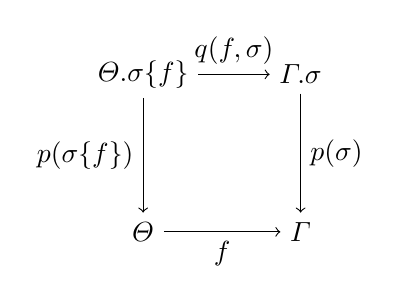
\begin{tikzpicture}
                \node(Bs) at (-1,  1) {$\Theta.\sigma\{f\}$};
                \node(Gs) at ( 1,  1) {$\Gamma.\sigma$};
                \node(B)  at (-1, -1) {$\Theta$};
                \node(G)  at ( 1, -1) {$\Gamma$};
        
                \draw[->] (Bs) to node[above] {$q(f, \sigma)$} (Gs);
                \draw[->] (Gs) to node[right] {$p(\sigma)$} (G);
                \draw[->] (Bs) to node[left]  {$p(\sigma\{f\})$} (B);
                \draw[->] (B)  to node[below] {$f$} (G);
            \end{tikzpicture}
        \end{center}

        such that $\qq(id_\Gamma,\sigma) = id_{\Gamma.\sigma}$ and $\qq(f\circ g,\sigma) = \qq(f,\sigma)\circ\qq(g,\sigma\{f\})$.
    \end{frame}

    % frame 20
    \section{Bonus}

    % frame 21
    \subsection{$\prod$ Type former}
    \begin{frame}
        \frametitle{$\prod$ Type former}
        \begin{itemize}
            \item Type former for the functions with return type depending on the parameter
            \item \underline{Set-theoretic equivalent:}\\
            Cartesian product over a family of sets: $\Pi_{i\in I}B_i$
            \item preserved by definitional equality
        \end{itemize}
        \vspace{40pt}
        $$\frac{\Gamma \vdash \sigma \typ \quad \Gamma,x:\sigma\vdash \tau \typ}{\Gamma \vdash \Pi x:\sigma.\tau \typ}\F$$
    \end{frame}

    % frame 22
    \begin{frame}
        \frametitle{$\Pi$ Rules}
        $$\frac{\Gamma, x:\sigma \vdash M : \tau}{\Gamma \vdash \lambda x:\sigma.M^\tau : \Pi x:\sigma.\tau}\Intro$$
        \vspace{20pt}
        $$\frac{\Gamma \vdash M : \Pi x: \sigma . \tau \quad \Gamma \vdash N: \sigma}{\Gamma \vdash \app{M}{N}: \tau[N/x]}\E$$
        \vspace{20pt}
        $$\frac{\Gamma \vdash \lambda x:\sigma.M^\tau:\Pi x:\sigma.\tau \quad \Gamma \vdash N:\sigma}{\Gamma \vdash \app{\lambda x:\sigma.M^{\tau}}{N} = M[N/x]:\tau[N/x]}\C$$
    \end{frame}

    \subsection{Interpretation}
    % frame 23
    \begin{frame}
        \frametitle{$\Pi$ type former interpretation}
        For each $\sigma\in Ty(\Gamma)$, $\tau\in Ty(\extension)$, $L\in Tm(\extension,\tau)$, $M\in Tm(\Gamma,\Pi(\sigma,\tau))$ and $N\in Tm(\Gamma,\sigma)$ we can define:
        \begin{itemize}
            \item the type $\Pi(\sigma,\tau)\in Ty(\Gamma)$
            \item the term $\lambda_{\sigma,\tau}(L)\in Tm(\Gamma,\Pi(\sigma,\tau))$
            \item the term $App_{\sigma,\tau}(M,N)\in Tm(\Gamma,\tau\{\Mbar\})$
        \end{itemize}
        such that
        \begin{align*}
            App_{\sigma,\tau}(\lambda_{\sigma,\tau}(M),N) &= M\{\overline{N}\} &\Pi-C\\
            \Pi(\sigma,\tau)\{f\} &= \Pi(\sigma\{f\},\tau\{\qq(f, \sigma)\}) &\Pi-S\\
            \lambda_{\sigma,\tau}(M)\{f\} &= \lambda_{\sigma\{f\},\tau\{\qq(f, \sigma)\}}(M\{\qq(f,\sigma)\}) &\lambda-S\\
            App_{\sigma,\tau}(M,N)\{f\} &= App_{\sigma\{f\},\tau\{\qq(f, \sigma)\}}(M\{f\},N\{f\}) &App-S
        \end{align*}
    \end{frame}

    % frame 24
    \begin{frame}
        \frametitle{Interpretation function}
        Let $\Brackets{-}$ an interpretation function such that:
        \begin{align*}
            \Brackets{\diamond} &= \top\\
            \Brackets{\Gamma,x:\sigma} &= \Brackets{\Gamma}.\Brackets{\Gamma;\sigma} &\text{if $x \not\in\Gamma$, undefined otherwise}\\
            \Brackets{\Gamma;\Pi x:\sigma.\tau} &= \Pi(\Brackets{\Gamma;\sigma},\Brackets{\Gamma,x:\sigma;\tau})\\
            \Brackets{\Gamma,x:\sigma;x} &= \texttt{v}_{\Brackets{\Gamma;\sigma}}\\
            \Brackets{\Gamma,x:\sigma,\Delta,y:\tau;x} &= \Brackets{\Gamma,x:\sigma,\Delta;x}\{\pp(\Brackets{\Gamma,x:\sigma,\Delta;\tau})\}\\
            \Brackets{\Gamma;App_{\sigma,[x:\sigma]\tau}(M,N)} &= App_{\Brackets{\Gamma;\sigma},\Brackets{\Gamma,x:\sigma;\tau}}(\Brackets{\Gamma;M},\Brackets{\Gamma;N})\\
            \Brackets{\Gamma;\lambda x:\sigma.M^\tau} &= \lambda_{\Brackets{\Gamma;\sigma},\Brackets{\Gamma,x:\sigma;\tau}}(\Brackets{\Gamma,x:\sigma;M})
        \end{align*}
    \end{frame}

    % frame 25
    \begin{frame}
        \frametitle{Soundness properties}
        \begin{align*}
            \Gamdash &\soundness \Brackets{\Gamma}\in\cate\\
            \Gamdash \sigma &\soundness \Brackets{\Gamma;\sigma}\in Ty(\Brackets{\Gamma})\\
            \Gamdash M:\sigma &\soundness \Brackets{\Gamma;M}\in Tm(\Brackets{\Gamma;\sigma})\\
            \vdash\Gamma = \Delta \cntxt &\soundness\Brackets{\Gamma}=\Brackets{\Delta}\\
            \Gamdash\sigma=\tau\typ&\soundness\Brackets{\Gamma;\sigma}=\Brackets{\Gamma;\tau}\\
            \Gamdash M = N:\sigma&\soundness\Brackets{\Gamma;M}=\Brackets{\Gamma;N}
        \end{align*}
    \end{frame}

    % % frame (27)
    % \begin{frame}
    %     \frametitle{Sections}
    %     Let $M \in Tm(\Gamma,\sigma) = Tm(\Gamma, \sigma\{id_\Gamma\})$\\
    %     \vspace{5pt}
    %     We can define a section of $\pp(\sigma)$ as
    %     $$\Mbar \defeq \langle id_\Gamma,M\rangle_\sigma:\Gamma\to\extension$$
    %     because the following statement holds:
    %     $$\pp(\sigma)\circ\Mbar =id_\Gamma$$
    %     \vspace{7pt}\\
    %     $Sect(\pp(\sigma))$ denotes the collection of sections of $\pp(\sigma)$.
    % \end{frame}
\end{document}